\documentclass[a4paper]{ctexart}

\usepackage{fancyhdr}
\usepackage{listings}
\usepackage{xcolor}
\usepackage{amsmath}
\usepackage{algorithm}
\usepackage{graphicx}
\usepackage[noend]{algpseudocode}
\usepackage{physics}
\usepackage{multirow}

% Codes settings
\lstset{
	language=Python,
	numbers = left,
	numberstyle = \tiny,
	basicstyle = \small,
	keywordstyle = \color{blue!70}\bfseries,
	stringstyle = \color{red},
	commentstyle =\color[rgb]{0.6,.6,.6}\itshape,
	identifierstyle={},
	frame = shadowbox,
	rulesepcolor= \color{ red!20!green!20!blue!20},
	escapeinside=``
}

%Page setting
\pagestyle{fancy}
\rfoot{\thepage}
\cfoot{}
\lfoot{\itshape Jeffreyyao@pku.edu.cn}
\setlength{\abovecaptionskip}{0.05cm}
\setlength{\belowcaptionskip}{0.05cm}

\title{计算物理第二次开卷考试}
\author{姚铭星 1700011321}
\date{}

\begin{document}
\maketitle
\tableofcontents
\section{马修方程}
\subsection{问题描述}
在离子阱,椭圆鼓的运动,射频四极矩,浮体的稳定性等问题中等等物理场景中,马修方程(Mathieu Equation)都发挥着重要的作用。本题的目标是求出马修方程的本征值。正则形式的马修方程:
\begin{equation}
-\frac{d^{2} \Psi(\phi)}{d \phi^{2}}+2 q \cos (2 \phi) \Psi(\phi)=A \Psi(\phi)\label{mathieu}
\end{equation}
在基于傅里叶基矢选取基函数为:
\begin{equation}
f_{k}(\phi)=\frac{1}{2 M+1} \sum_{n=-M}^{n=M} \Phi_{n}^{*}\left(\phi_{k}\right) \Phi_{n}(\phi)
\end{equation}
这时方程(\ref{mathieu})在这组基矢下可以被重新写为:
\begin{equation}
\mathbf{H} \Psi=[\mathbf{T}+\mathbf{V}] \Psi=A \Psi\label{Newmathieu}
\end{equation}
其中$A$为马修方程的本征值。
\subsection{QR分解算法}
方程(\ref{Newmathieu})中的矩阵$H$是稠密矩阵,因此本征值用QR分解的方法最为合适。
算法是基于讲义的倒数第2、3页完成的。

\textbf{Householder变换}:
\begin{lstlisting}
def Householder(A):
	'''
	Householder变换,返回Hessengerg矩阵和变换矩阵(A,G)
	输入A:矩阵
	'''
	n = A.shape[0]
	P = np.identity(n)
	for i in range(n-2):
		# 构建反射矩阵
		x = A[i+1:,i] # 取矩阵列共(n-i-1)维
		e = np.array([1]+[0 for x in range(n-i-2)]) # 构造单位矢量
		v = np.sign(x[0])*norm(x)*e+x # 构造反射矢量
		v = v/norm(v) #归一化 
		G = np.array([[2*x*y for x in v]for y in v])
		H = lin.block_diag(np.identity(i+1),np.identity(n-i-1)-G)# 构建反射矩阵
		A = H@A@H
		P = H@P
	return A,P
\end{lstlisting}

\textbf{QR分解}:
\begin{lstlisting}
def decompose(A):
	'''
	利用Givens变换分解,A为上海森堡矩阵
	返回(Q,R)
	'''
	n = A.shape[0]
	G = np.identity(n) # Givens 矩阵
	for i in range(n-1): # 共(n-1)个非对角元需要消去
		cos = A[i,i]/np.sqrt(A[i,i]**2+A[i+1,i]**2)
		sin = A[i+1,i]/np.sqrt(A[i,i]**2+A[i+1,i]**2)
		G1 = lin.block_diag(np.identity(i),np.array([[cos,sin],[-sin,cos]]),np.identity(n-i-2))
		A = G1@A
		G = G@G1.T
	return G , A
\end{lstlisting}

\textbf{QR算法:}
\begin{lstlisting}
def QR(A):
	'''
	QR算法,输入Hessengberg矩阵A
	返回特征值和特征向量
	'''
	n = A.shape[0]
	i = 0
	N = 10**5
	e = 10**(-8)
	# G = np.identity(n)
	k = n-1
	res = [] # 储存本征矢量
	while k > 0:
		if abs(A[k,k-1])<e: # 本征值必然是实数
		res.append(A[k,k]) # 本征值代入
		A = A[:k,:k] # 取子阵
		k = k-1
		s = A[k,k] # 位移因子
		A=A-s*np.identity(k+1)
		Q, R = decompose(A)
		A = R@Q + s*np.identity(k+1)
		i+=1
		if i > N: 
			raise("Too many Loops!")
	res.append(A[0,0])# 加入最后一个本征值
	return res
\end{lstlisting}
\subsection{本征值图线}
计算出的前11个本征值如图(绘图调用了\textit{matplotlib.pyplot}方法)
\begin{figure}[hbt]
	\centering
	\includegraphics[width=8cm]{./fig/eigen_1.png}
	\caption{前11个本征值随q的变化关系}
\end{figure}
\subsection{偶宇称解}
不难证明:
\begin{equation}
f_k(-\phi)=f_{2M+1-k}(\phi)
\end{equation}
因此,有:
\begin{equation}
\begin{aligned}
\Psi(-\phi)&=\sum_{k=1}^{2 M+1} C_{k} f_{k}(-\phi)\\
&=\Psi(-\phi)=\sum_{k=1}^{2 M+1} C_{k} f_{2M+1-k}(\phi)
\end{aligned}
\end{equation}
判断奇偶宇称的方式为判断$C_k$和$C_{2M+1-k}$的关系。
注意到当$q=0$时会出现简并现象,实际上,可以通过重新线性组合的方式,得到新的满足宇称对称性的解
\begin{equation}
\left\{\begin{array}{l}{\frac{1}{2}(\Psi(\phi)+\Psi(-\phi))},\qquad \text{Even} \\ {\frac{1}{2}(\Psi(\phi)-\Psi(-\phi))}\qquad \text{Odd}\end{array}\right.
\end{equation}
\begin{figure}[hbt]
	\centering
	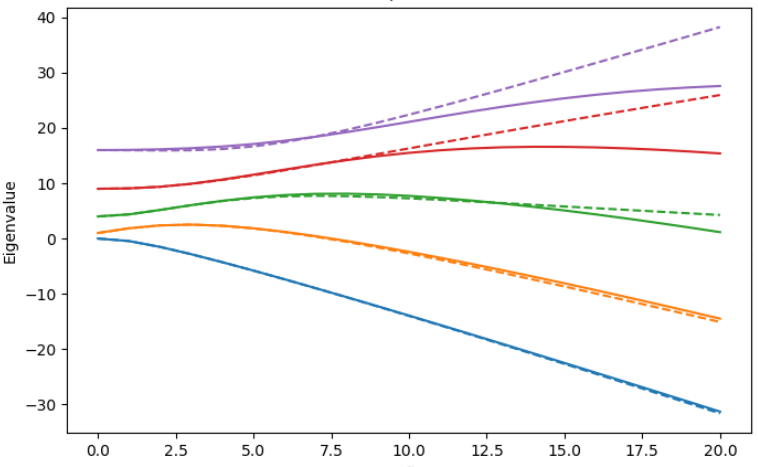
\includegraphics[width=8cm]{./fig/Eigen_2.png}
	\caption{虚线为M=5,实线为M=40}
\end{figure}

\subsection{$M=50$,$q=10$的情况}
直接按上问的方法求解出本征值:
\begin{figure}[hbt]
	\centering
	\includegraphics[width=12cm]{./fig/eigen_3.png}
\end{figure}
由于存在以下关系式
可以直接画图
\begin{equation}
C_{k}=2 \pi \Psi\left(\phi_{k}\right)=2 \pi \Psi\left(\phi_{k}-2 \pi\right)
\end{equation}
\begin{figure}[hbt]
	\centering
	\includegraphics[width=12cm]{./fig/eigen_4.png}
	\caption{前六个本征矢和}
\end{figure}
实际上由于利用正交矩阵求出的本征矢量误差较大,实际上可以使用反幂法来利用本征值迭代得到本征矢。
\section{氢原子电离}
\subsection{鞍点法近似}
题文的背景为求解氢原子的跃迁问题,即电子从束缚态跃迁到自由态的问题。问题的关键是求解跃迁矩阵元:
\begin{equation}
\begin{aligned} M_{\mathbf{p}}^{0}\left(t_{f}, t_{i}\right)_{D I} &=\int_{t_{i}}^{t_{f}} d t\left\{\frac{\partial}{\partial \mathbf{q}}\left[\frac{2^{\frac{3}{2}}\left(2 I_{p}\right)^{\frac{5}{4}}}{\pi\left(\mathbf{q}^{2}+2 I_{p}\right)^{2}}\right]\right\} \cdot \mathbf{E}(t) e^{i S(t)} \\ &=2^{\frac{7}{2}}\left(2 I_{p}\right)^{\frac{5}{4}} \int_{t_{i}}^{t_{f}} d t \frac{\mathbf{q} \cdot \mathbf{E}(t)}{\pi\left(\mathbf{q}^{2}+2 I_{p}\right)^{3}} e^{i S(t)} \\
S(t)&=\int_{0}^{t} d \tau\left[\frac{1}{2}(\mathbf{p}+\mathbf{A}(\tau))^{2}+I_{p}\right]\end{aligned}
\end{equation}

求解给定动量$p$下的鞍点方程:
\begin{equation}
\frac{\partial S(t)}{\partial t}=0, \quad \quad t=t_{s}=t_{r}+i t_{i}
\end{equation}
从而得到鞍点法近似下的积分近似值:
\begin{equation}
M_{\mathrm{p}}^{0}\left(t_{f}, t_{i}\right)_{S P M}=-\frac{\left(2 I_{p}\right)^{\frac{5}{4}}}{\sqrt{2}} \sum_{\alpha} \frac{1}{S^{\prime \prime}\left(t_{s \alpha}\right)} e^{i S\left(t_{s \alpha}\right)}
\end{equation}
其中求和为对所有物理解($Im(t_{\alpha})>0$)的鞍点$\alpha$求和。

\subsubsection{非线性方程求根}
为了简单起见,下面记$B=\frac{A_0}{2}$.鞍点方程:
\begin{equation}
0=\frac{1}{2} q\left(t_{s \alpha}\right)^{2}+I_{p}=\frac{1}{2}\left(B \sin \tau\left.\left(1-\cos \frac{\tau}{2}\right)\right|_{\tau=\omega t_{s \alpha}}+p_{z}\right)^{2}+I_{p}\label{1}
\end{equation}
通过代换$x=e^{i\tau/2}$可以将上方程变为两个一元六次方程:
\begin{equation}
x^{6}-2 x^{5}+x^{4}+D_{ \pm} x^{3}-x^{2}+2 x-1=0, \quad D_{ \pm}=\frac{4}{B}\left(\mp \sqrt{2 I_{p}}-\mathrm{i} p_{z}\right)
\end{equation}
由于方程\ref{1}是一个实数方程,两个方程的六个根互为共轭关系,因此我们只需要求解$D_+$的六个解,如果得到了$\operatorname{Im} t_{s \alpha}<0$的根,只需要进行对实轴的镜像对称即可(取共轭)。解出$x$之后只需要进行$\tau=\frac{2}{i}\ln(x)$,$t_\alpha=\tau/\omega$

当求解出所有的根之后,在进行鞍点法积分时还会用到$S(t_\alpha)$和$S''(t_\alpha)$,它们都可以解析地求出:
\begin{equation}
\partial_{t}^{2} S(t)=\omega \partial_{\tau} g(\tau)=\omega q(\tau) \partial_{\tau} A(\tau)
\end{equation}
\begin{equation}
\begin{aligned} q(\tau) &=B \sin \tau\left(1-\cos \frac{\tau}{2}\right)+p_{z} \\ \partial_{\tau} A(\tau) &=B\left(\cos \tau\left(1-\cos \frac{\tau}{2}\right)+\frac{1}{2} \sin \tau \sin \frac{\tau}{2}\right) \end{aligned}
\end{equation}
\begin{equation}\begin{aligned} \omega S\left(\frac{\tau}{\omega}\right)=&\left(\frac{3}{8} B^{2}+\frac{1}{8} p_{z}^{2}+I_{p}\right) \tau-\frac{1}{3} B p_{z}+B p_{z}\left(\cos \frac{\tau}{2}-\cos \tau+\frac{1}{3} \cos \frac{3 \tau}{2}\right) \\ &-B^{2}\left(\sin \frac{\tau}{2}-\frac{1}{16} \sin \tau-\frac{1}{6} \sin \frac{3 \tau}{2}+\frac{3}{16} \sin (2 \tau)-\frac{1}{10} \sin \frac{5 \tau}{2}\right.\\ &\left. +\frac{1}{48} \sin (3 \tau) \right) \end{aligned}
\end{equation}
\subsubsection{代码实现}
多项式求复数根采用的为牛顿收缩法,从而求得多项式方程的所有复数根。为了更好地选取初始的猜测解的位置,首先先画个图看一看根的分布。
\begin{figure}[hbt]
\centering
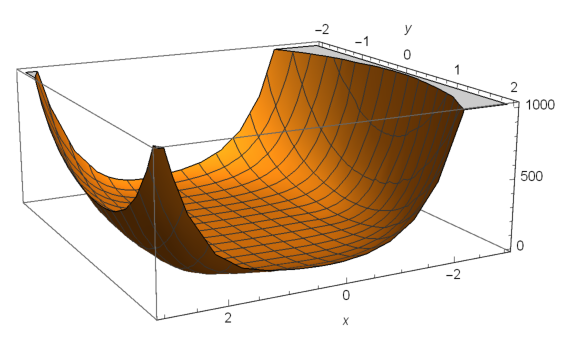
\includegraphics[width=5cm]{./fig/plot_1.eps}
\end{figure}
可以看到,当x的实部和虚部超过2时,函数的模值将超过100。由Cauthy定理,可以合理猜测根的范围大致在2以内,因此初始化的随机数生成根的范围为实部和虚部均小于2的实数。
\begin{lstlisting}
def rand():
	return 4*np.random.random_sample()-2

def Newton_deflation(a,N=10**3,e=10**(-14)):
	'''
	牛顿法解方程
	输入a为多项式类<class 'numpy.poly1d'>
	N为最大迭代次数,e为迭代精度
	返回一个根和收缩多项式
	'''
	n = 0
	x = complex(rand(),rand())# 初始取值
	while n<N:# 控制迭代次数
		d = np.poly1d((1,-x))
		q , b = a/d # numpy.poly1d中已经重载运算符
		if abs(b[0])<e: # 当余项小于某一上界
			# print(b)
			return x, q
		x-=b[0]/q(x) # 牛顿法q(x)即为多项式的导数
	else:
		print(str(n)+" loops")
		return x, q
\end{lstlisting}
鞍点法求出的根为:

\begin{figure}[hbt]
	\centering
	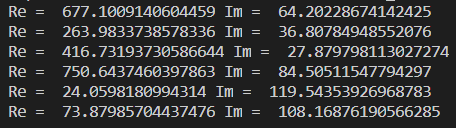
\includegraphics[width=12cm]{./fig/SPM_1.png}
\end{figure}
为了能体现出振荡的效果,在区间内取了$100$个数据点
\begin{figure}[hbt]
	\centering
	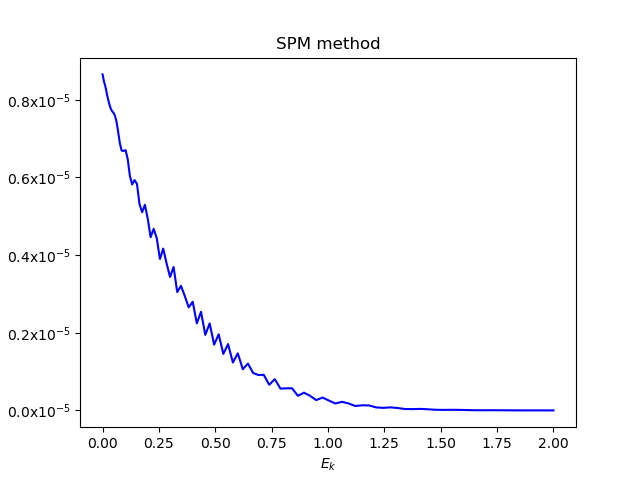
\includegraphics[width=12cm]{./fig/SPM_2.png}
	\caption{鞍点法导出的色散关系}
\end{figure}
\subsection{直接积分法}
实际上直接积分也能求解出矩阵元
\begin{equation}
M_{\mathbf{p}}^{0}\left(t_{f}, t_{i}\right)=\frac{2^{7 / 2}\left(2 I_{p}\right)^{5 / 4}}{\pi} \int_{t_{i}}^{t_{f}} \mathrm{d} \tau \frac{-q(\tau) \partial_{\tau} A(\tau)}{\left(q(\tau)^{2}+2 I_{p}\right)^{3}} \mathrm{e}^{\mathrm{i} S(\tau / \omega)}
\end{equation}
其中$q(\tau), \partial_{\tau} A(\tau), S(t)$在之前已经求出。接下来可以直接用复化梯形求积公式计算
\begin{equation}
\begin{array}{l}{T_{n}=\sum_{k=0}^{n-1} \frac{h}{2}\left[f\left(x_{k}\right)+f\left(x_{k+1}\right)\right]} \\ {=\frac{h}{2}\left\{\left[f(a)+f\left(x_{1}\right)\right]+\left[f\left(x_{1}\right)+f\left(x_{2}\right)\right]+\cdots+\left[f\left(x_{n-1}\right)+f(b)\right]\right\}} \\ {=\frac{h}{2}\left[f(a)+2 \sum_{k=1}^{n-1} f\left(x_{k}\right)+f(b)\right]}\end{array}
\end{equation}
\begin{equation}
T_{2 n}=\frac{T_{n}}{2}+\frac{h}{2} \sum_{k=0}^{n-1} f\left(x_{k+\frac{1}{2}}\right)
\end{equation}
其中积分间隔为$h=\frac{b-a}{n}$

\subsection{结果展示}
\begin{figure}[hbt]
	\centering
	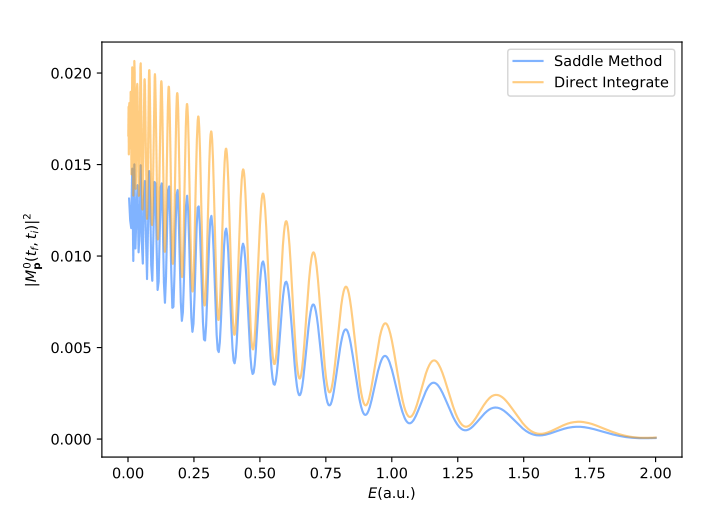
\includegraphics[width=12cm]{./fig/SPM_3.png}
	\caption{直接积分和鞍点法的比较}
\end{figure}
注意,上面的绝对数值并不正确。
\section{第三题:随机游走问题}
由于此题小问较多,下面逐问回答
\subsection{第一问}
设$s=1-p-q$为原地不动的概率:
则有如下几种情况:
\begin{enumerate}
	\item 到达+3的概率:$p^3$
	\item 到达+2的概率:$\left( \begin{array}{l}{3} \\ {1}\end{array}\right) p^{2} s$
	\item 到达+1的概率:$\left( \begin{array}{l}{3} \\ {1}\end{array}\right) p s^{2}+\left( \begin{array}{l}{3} \\ {1}\end{array}\right) p^{2} q$
	\item 原地不动的概率:$s^3$
	\item 到达-1的概率:$\left( \begin{array}{l}{3} \\ {1}\end{array}\right) q s^{2}+\left( \begin{array}{l}{3} \\ {1}\end{array}\right) q^{2} p$
	\item 到达-2的概率:$\left( \begin{array}{l}{3} \\ {1}\end{array}\right) q^{2} s$
	\item 到达-3的概率:$q^3$
\end{enumerate}
根据期望的定义
\begin{equation}
E[x]=\sum_{x}|x| \operatorname{Pr}[x]=3((p+q)(1+2 p q)-4 p q)
\end{equation}
\subsection{第二问}
\subsubsection{伪随机数产生器}
伪随机采用线性同余产生器(LCG)方式产生
\begin{equation}
x_{n+1}=a x_{n}+c \quad(\bmod m)
\end{equation}
其中选取$a=1140678415$、$c=12345$和$m=2^{31}-1$,选取默认的发生种子$x_0$为时间戳。
\begin{lstlisting}
from time import time

def pseudo_rand(n=1,x0 = int(time())):
	'''
	线性同余伪随机数产生
	'''
	m = 2**31-1
	a = 1140678415
	c = 12345
	res = []
	for _ in range(n):
		x0 = (a*x0+c)%m
		res.append(x0)
    res = [float(each)/m for each in res]
	return res
\end{lstlisting}
结果保存在\textit{./res.txt}中
\subsection{第三问}
\subsubsection{代码实现}
\begin{lstlisting}
def Third_rand_walk(n=100):
	'''
	第三问
	'''
	a = pseudo_rand(n)
	# a = [np.random.random_sample() for _ in range(n)]
	sequ = [2*np.pi*each for each in a]
	x=y=0
	for each in sequ:
		x+=np.cos(each)
		y+=np.sin(each)
	return np.sqrt(x**2+y**2)
\end{lstlisting}
\subsubsection{拟合数据}
数据拟合采用正比拟合
\begin{equation}
\mathrm{E}[R]=a \sqrt{N}
\end{equation}
利用最小二乘法的公式:
\begin{equation}
a=\frac{\sum_{n} x_{n} y_{n}}{\sum_{n} x_{n}^{2}}
\end{equation}
\begin{equation}
r=\frac{\sum_{n} x_{n} y_{n}}{\sqrt{\sum_{n} x_{n}^{2} \sum_{n} y_{n}^{2}}}
\end{equation}
\subsubsection{结果展示}
计算结果得到:

\begin{figure}[hbt]
	\centering
	\includegraphics[width=5cm]{./fig/walk_res.png}
\end{figure}
讲拟合出来的直线和散点图绘制在同一张图上得到:
\begin{figure}[hbt]
	\centering
	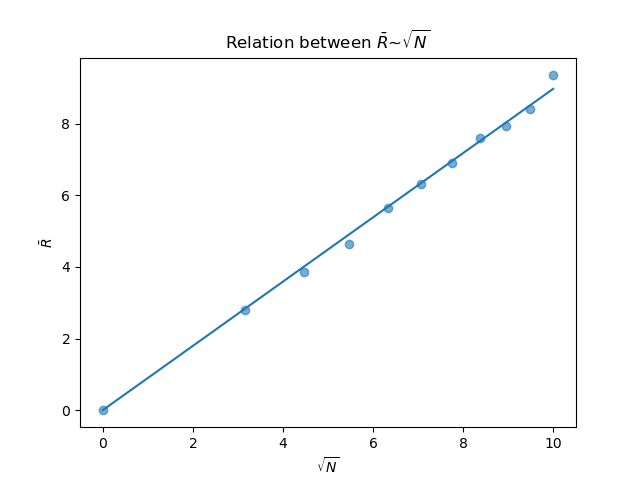
\includegraphics[width=8cm]{./fig/Walk_1.png}
\end{figure}
\subsection{第四问}
设$Z_n=X_n+iY_n$,有公式:
\begin{equation}
Z_{n}=\sum_{k} \mathrm{e}^{\mathrm{i} \theta_{k}}
\end{equation}
由于对于$\theta$是均匀分布的,有:
\begin{equation}
\mathrm{E}\left[\mathrm{e}^{\mathrm{i} \theta}\right]=\int_{0}^{2 \pi} \frac{\mathrm{d} \theta}{2 \pi} \mathrm{e}^{\mathrm{i} \theta}=0
\end{equation}
因此有:
\begin{equation}
\mathrm{E}\left[Z_{n}\right]=\sum_{k} 0=0
\end{equation}
这样可以导出
\begin{equation}
\mathrm{E}\left[X_{n}\right]=\mathrm{E}\left[Y_{n}\right]=0
\end{equation}
\textbf{方差计算}:
\begin{equation}
\begin{aligned}
Var(X_n)=E[X_n^2]&=\sum_{k=1}^{n}\sum_{l=1}^{n} E[\cos \theta_{k} \cos \theta_{l}]\\
&=\sum_{k=1}^{n}\frac{1}{2}=\frac{n}{2}
\end{aligned}
\end{equation}
同理可以计算得到
\begin{equation}
Var(Y_n)=\frac{n}{2}
\end{equation}
\subsection{第五问}
X,Y的相关性可以用协方差描述:
\begin{equation}
\begin{aligned}
Cov(X_n,Y_n)&=E[X_nY_n]-E[X_n]E[Y_n]\\
&=\sum_{k, \ell} \mathrm{E}\left[\cos \theta_{k} \sin \theta_{\ell}\right]
\end{aligned}
\end{equation}
分下面两种情况讨论
\begin{equation}
\left\{
\begin{array}{ll}{k \neq \ell,} & {\int_{0}^{2 \pi} \int_{0}^{2 \pi} \frac{\mathrm{d} \theta_{k}}{2 \pi} \frac{\mathrm{d} \theta_{\ell}}{2 \pi} \cos \theta_{k} \sin \theta_{\ell}=0} \\ {k=\ell,} & {\int_{0}^{2 \pi} \frac{\mathrm{d} \theta_{k}}{2 \pi} \cos \theta_{k} \sin \theta_{k}=0}\end{array}\right.
\end{equation}
故随机变量$X_n$与$Y_n$可视为独立
\subsection{第六问}
当$n\to\infty$时,根据中心极限定理,随机变量$\sqrt{n}\left(S_{n}-\mu\right)$收敛到多维正态分布$N(0,\Sigma)$
对题文中情况,为二维分布
\begin{equation}
N(\mu, \Sigma)=\frac{1}{\sqrt{(2 \pi)^{r}|\Sigma|}} \exp \left(-\frac{1}{2}(x-\mu)^{T} \Sigma^{-1}(x-\mu)\right)
\end{equation}
将之前计算的结果代入
\begin{equation}
\mu=\left( \begin{array}{l}{0} \\ {0}\end{array}\right) \quad \Sigma=\left( \begin{array}{ll}{\frac{1}{2}} & {0} \\ {0} & {\frac{1}{2}}\end{array}\right)
\end{equation}
得到
\begin{equation}f(x_n,y_n)
=\frac{1}{\sqrt{n \pi}} \exp \left(\frac{-x_{n}^{2}}{n}\right) \frac{1}{\sqrt{n \pi}} \exp \left(\frac{-y_{n}^{2}}{n}\right)
\end{equation}
\subsection{第七问}
将上一问中的直角坐标变换到柱坐标中,并且将角向的自由度积分后可以得到:
\begin{equation}
\begin{aligned}
f(\rho)d\rho &=\int_{0}^{2 \pi} \rho \mathrm{d} \rho \mathrm{d} \varphi \frac{1}{n \pi} \exp \left(-\frac{\rho^{2}}{n}\right)\\
f(\rho)&=\frac{2\rho}{n}\exp\left(-\frac{\rho^2}{n}\right)
\end{aligned}
\end{equation}
\subsection{第八问}
\begin{equation}
E[R_n]=\int_{0}^{\infty}\rho f(\rho)d\rho=\frac{\sqrt{\pi}}{2}\sqrt{n}\approx 0.886\sqrt{n}
\end{equation}
相差仅为约1.3\%
\end{document}